%%% TokenSmith course-project report
%%% ACM SIG Proceedings template (acmart, sigconf option)

\documentclass[sigconf]{acmart}

\usepackage{booktabs}
\usepackage{graphicx}
\usepackage{xcolor}
\usepackage{tikz}
\usetikzlibrary{positioning, arrows.meta, fit}

\newcommand{\shivam}[1]{\textcolor{teal}{[shivam: #1]}}

\setcopyright{none}
\acmConference[CS 6423]{CS 6423 Course Project}{Spring 2026}{Georgia Tech}
\acmDOI{}
\acmISBN{}
\settopmatter{printacmref=false, printccs=false, printfolios=true}

\begin{document}

\title{Optimizing TokenSmith for Consumer-GPU Hardware}

\author{Shivam Singhal}
\email{ssinghal88@gatech.edu}
\affiliation{%
  \institution{Georgia Institute of Technology}
  \city{Atlanta}
  \state{GA}
  \country{USA}
}
\renewcommand{\shortauthors}{Singhal}

\begin{abstract}
TokenSmith is a local-first RAG system for textbook question answering.
The original implementation is fully functional but is impractical for
a new user trying it on a fresh textbook, since cold ingestion before
the first answer takes close to three hours on a server and longer on
a laptop. We re-target the system for consumer hardware (one GPU with
at most 8\,GiB of memory, four CPU cores) by making four pipeline
changes: parallel PDF extraction, a \texttt{pypdfium2} fast extraction
path, a hardware-aware embedding router with length-sorted batches,
and a pluggable embedder that can target \texttt{llama.cpp}, GPT4All
(CUDA or Vulkan), or HuggingFace \texttt{sentence-transformers} at a
fixed call site. On a Quadro RTX 6000 capped at 8\,GiB, every variant
stays well under the cap. The most efficient configuration
(\texttt{pypdfium2} extractor + 23\,M MiniLM embedder) extracts the
2{,}195-page textbook in 8.66\,s, finishes embedding in about 30\,s,
and answers each query in about 3.7\,s, so cold ingestion-to-first-
answer is roughly 45 seconds on a 4-core / 8-GiB consumer machine. The
accuracy drop relative to the 4\,B baseline is 1.4 points on the
final score (0.578 vs.\ 0.592); the 4\,B baseline itself fits in
5.4\,GiB.
\end{abstract}

\keywords{retrieval-augmented generation, local inference, embeddings,
consumer GPU, FAISS}

\maketitle

%% ------------------------------------------------------------
\section{Introduction}

The original TokenSmith assumes a server with a large GPU. The cold
ingestion path (extract a PDF to markdown, chunk, embed, build FAISS
and BM25) dominates time-to-first-token. On a 64-core server the
sequential \texttt{docling} extraction of the 2{,}195-page Silberschatz
\emph{Database System Concepts} textbook alone takes about 9{,}650\,s
(close to 2 hours and 40 minutes), while the rest of the cores sit
idle. Indexing adds another 5 to 7 minutes on a server GPU (305\,s on
A100, 426\,s on V100), and several hours on a CPU-only host (the
GPT4All Nomic backend takes a projected 7{,}212\,s on the same corpus
without a GPU). Indexing is dominated by the 4\,B \texttt{Qwen3-Embedding}
model. Retrieval and generation take about 3 to 4 seconds per query
on the same hardware. A new user pointing TokenSmith at a fresh textbook
therefore waits multiple hours before the first answer comes back.

On a 4-core laptop with the original sequential code, the picture is
worse. Extraction runs at single-core speed (about 9{,}650\,s per
textbook, since each \texttt{docling} worker pegs one core regardless
of host CPU count); indexing on a consumer GPU like the RTX 6000 adds
roughly 30 to 60 seconds once the model is loaded; the first answer
takes about 4\,s. Cold time-to-first-token is therefore close to 2
hours and 45 minutes on a laptop. The system works, but in practice
no student would sit through a first run.

The goal of this project is to make ingestion fast enough that a
student can drop a new PDF in and get a useful answer in the same
study session, without sending data off the host. We use the
Silberschatz textbook as the canonical corpus (2{,}195 pages, 2{,}664
chunks after section-aware splitting) and target a consumer machine
with at most 8\,GiB of GPU memory and four CPU cores. Our most
efficient configuration peaks at roughly 3\,GiB of host RAM and 2\,GiB
of GPU memory during a full ingestion; the heaviest variant (the 4\,B
GGUF embedder plus the 1.5\,B generator, both on GPU) peaks at
5.4\,GiB of GPU memory.

%% ------------------------------------------------------------
\section{System Pipeline and Evaluation Metrics}
\label{sec:system}

\subsection{Pipeline}

Figure~\ref{fig:pipeline} shows the TokenSmith pipeline. It splits
into a \emph{cold ingestion} path that runs once per textbook and a
\emph{per-query} path that runs every time a student asks a question.

\begin{figure*}[t]
\centering
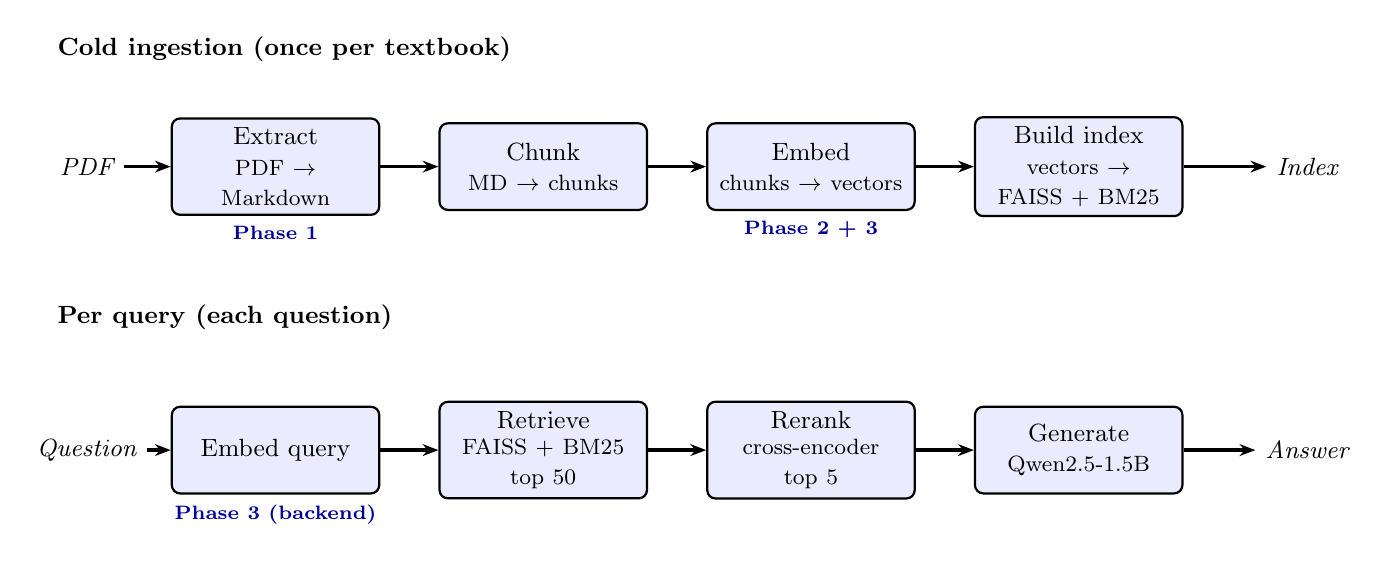
\begin{tikzpicture}[
  > = {Stealth[length=2mm]},
  thick,
  font=\small,
  stage/.style={draw, rounded corners=3pt, fill=blue!8,
                minimum height=11mm, text width=24mm, align=center},
  io/.style={font=\small\itshape, align=center},
  arr/.style={->, very thick}
]
  % --- Cold ingestion row label (placed clearly above the boxes) ---
  \node[font=\small\bfseries, anchor=south west]
    at (-0.5, 1.2) {Cold ingestion (once per textbook)};

  % --- Cold ingestion row ---
  \node[io]    (pdf) at (0, 0)     {PDF};
  \node[stage] (ext) at (2.4, 0)   {Extract\\\footnotesize PDF $\to$ Markdown};
  \node[stage] (chk) at (5.8, 0)   {Chunk\\\footnotesize MD $\to$ chunks};
  \node[stage] (emb) at (9.2, 0)   {Embed\\\footnotesize chunks $\to$ vectors};
  \node[stage] (idx) at (12.6, 0)  {Build index\\\footnotesize vectors $\to$ FAISS + BM25};
  \node[io]    (db)  at (15.5, 0)  {Index};

  \draw[arr] (pdf) -- (ext);
  \draw[arr] (ext) -- (chk);
  \draw[arr] (chk) -- (emb);
  \draw[arr] (emb) -- (idx);
  \draw[arr] (idx) -- (db);

  \node[font=\scriptsize\bfseries, color=blue!60!black,
        anchor=north] at (ext.south) {Phase 1};
  \node[font=\scriptsize\bfseries, color=blue!60!black,
        anchor=north] at (emb.south) {Phase 2 + 3};

  % --- Per-query row label (placed clearly above its boxes) ---
  \node[font=\small\bfseries, anchor=south west]
    at (-0.5, -2.2) {Per query (each question)};

  % --- Per-query row ---
  \node[io]    (q)   at (0, -3.6)  {Question};
  \node[stage] (qe)  at (2.4, -3.6){Embed query};
  \node[stage] (ret) at (5.8, -3.6){Retrieve\\\footnotesize FAISS + BM25\\\footnotesize top 50};
  \node[stage] (rer) at (9.2, -3.6){Rerank\\\footnotesize cross-encoder\\\footnotesize top 5};
  \node[stage] (gen) at (12.6, -3.6){Generate\\\footnotesize Qwen2.5-1.5B};
  \node[io]    (a)   at (15.5, -3.6){Answer};

  \draw[arr] (q)   -- (qe);
  \draw[arr] (qe)  -- (ret);
  \draw[arr] (ret) -- (rer);
  \draw[arr] (rer) -- (gen);
  \draw[arr] (gen) -- (a);

  \node[font=\scriptsize\bfseries, color=blue!60!black,
        anchor=north] at (qe.south) {Phase 3 (backend)};
\end{tikzpicture}
\caption{TokenSmith pipeline. The cold ingestion path (top) runs once
per textbook and produces a FAISS + BM25 index over section-aware
chunks. The per-query path (bottom) embeds the question, retrieves
the 50 nearest chunks, reranks them with a cross-encoder, prompts the
1.5\,B Qwen2.5 generator. Phases 1 to 3 all attack the cold path; the
per-query path is unchanged in cost (about 3.5\,s end to end on the
consumer GPU). Phase 3's pluggable embedder also reaches the per-query
\textsc{embed} stage because the same backend that built the index is
used to embed the question.}
\label{fig:pipeline}
\end{figure*}

Table~\ref{tab:pipeline-summary} lists the wall time per stage on the
consumer profile (4 CPU cores, RTX 6000 with the 8\,GiB cap), so the
cost of each box in Figure~\ref{fig:pipeline} is concrete. The cold
path goes from close to three hours on the unoptimized code to about
45 seconds end to end on the optimized pipeline; the per-query path
was already fast and we leave it alone.

\begin{table}[h]
\caption{Per-stage wall time on the consumer profile (4-core,
RTX 6000, 8\,GiB cap), most efficient configuration.}
\label{tab:pipeline-summary}
\begin{tabular}{llrr}
\toprule
Stage              & Phase     & Baseline       & Optimized \\
\midrule
\multicolumn{4}{l}{\emph{Cold ingestion (per textbook)}} \\
\quad Extract      & 1         & 9{,}650\,s     & \textbf{8.66\,s} \\
\quad Chunk        & ---       & $<$1\,s        & $<$1\,s \\
\quad Embed        & 2, 3      & 426\,s         & \textbf{$\sim$30\,s} \\
\quad Build index  & ---       & $<$5\,s        & $<$5\,s \\
\midrule
\multicolumn{4}{l}{\emph{Per query}} \\
\quad Embed query  & 3 (bk)    & $\sim$1\,ms    & $\sim$1\,ms \\
\quad Retrieve     & ---       & $<$100\,ms     & $<$100\,ms \\
\quad Rerank       & ---       & $\sim$0.5\,s   & $\sim$0.5\,s \\
\quad Generate     & ---       & $\sim$3\,s     & $\sim$3\,s \\
\midrule
\textbf{Cold TTFT} &           & \textbf{$\sim$2\,h\,48\,m} & \textbf{$\sim$45\,s} \\
\bottomrule
\end{tabular}
\end{table}

\subsection{Evaluation Metrics}
\label{sec:metrics}

We evaluate every change against the same 11-question benchmark suite
present in the project's repository. Each benchmark has a hand-written
reference answer. We report four quality numbers per variant and two
resource numbers.

\begin{description}
\item[Semantic similarity (sem).] Cosine similarity between the
  \texttt{all-mpnet-base-v2} embedding of the generated answer and that
  of the reference answer. Range $[0, 1]$, higher is better. Captures
  whether the answer means the same thing as the reference, even when
  the wording differs.

\item[Keyword similarity (kw).] Fraction of reference-answer keywords
  that appear in the generated answer. Range $[0, 1]$, higher is
  better. Captures whether the right technical terms made it into the
  answer.

\item[BLEU.] Sentence-level BLEU-4 with NIST method-1 smoothing on the
  lowercased, tokenized answer pair. Range $[0, 1]$, higher is better.
  Captures how much the answer overlaps with the reference at the
  surface phrase level.

\item[Final score.] Weighted mean of the three above:
  $0.5 \cdot \text{sem} + 0.3 \cdot \text{kw} + 0.2 \cdot \text{BLEU}$.
  This is the single number we use to rank variants. Range $[0, 1]$,
  higher is better.

\item[Peak VRAM.] Maximum GPU memory in use at any point during the
  run, in MiB. Reported by sampling \texttt{nvidia-smi} every
  500\,ms. The headline target is staying under the 8\,GiB cap.

\item[Wall time.] Seconds from the start of the test run to the last
  benchmark finishing. For Phase 2 we report the embedding step in
  isolation; for Phase 3 we report the full per-question loop
  (embed query, retrieve, rerank, generate, score) summed over all
  11 benchmarks.
\end{description}

%% ------------------------------------------------------------
\section{Phase 1: Faster PDF Extraction}

The single largest contributor to time-to-first-token is PDF
extraction. We attack it twice. First by parallelizing the existing
\texttt{docling} backend across CPU workers, then by replacing the
backend itself for plain-text textbooks where layout analysis is
unnecessary.

\subsection{Map-Reduce Architecture for Extraction}

The original extractor calls \texttt{docling} on the full PDF in a
single pass. Page-level layout analysis is the slow part of
\texttt{docling}, and it is independent across pages, so we restructure
extraction as a map-reduce pipeline.

In the map phase, the master PDF is split into fixed-size page-range
chunks. Each chunk is dispatched to its own worker process, which
loads its own \texttt{docling} instance, converts the chunk to
markdown, and returns the markdown along with the chunk's start-page
offset. Workers run inside a process pool sized to the available CPU
count. In the reduce phase, the per-worker outputs are sorted on
offset and concatenated into a single markdown document. Loading
\texttt{docling} costs about 100\,MB per process; we defer that import
into the worker function so callers that import the extractor without
actually using it (the indexer, the test harness) skip the cost.

We swept the worker count on a 64-core server in
$\{1, 2, 4, 8, 16, 32, 62\}$. Table~\ref{tab:phase1} reports the
total wall time per configuration; Figure~\ref{fig:extraction-scaling}
plots the same data on a log y-axis.

\begin{table}[h]
\caption{Phase 1: docling extraction on the 2{,}195-page textbook
(64-core server host).}
\label{tab:phase1}
\begin{tabular}{lrrrrrrr}
\toprule
workers   & 1       & 2       & 4       & 8       & 16      & 32      & 62 \\
\midrule
wall (s)  & 9{,}650 & 4{,}289 & 2{,}018 & 2{,}252 & 1{,}116 & 535     & 382 \\
speedup   & 1.0$\times$ & 2.3$\times$ & 4.8$\times$ & 4.3$\times$ & 8.7$\times$ & 18.0$\times$ & \textbf{25.3$\times$} \\
\bottomrule
\end{tabular}
\end{table}

\begin{figure}[h]
\centering
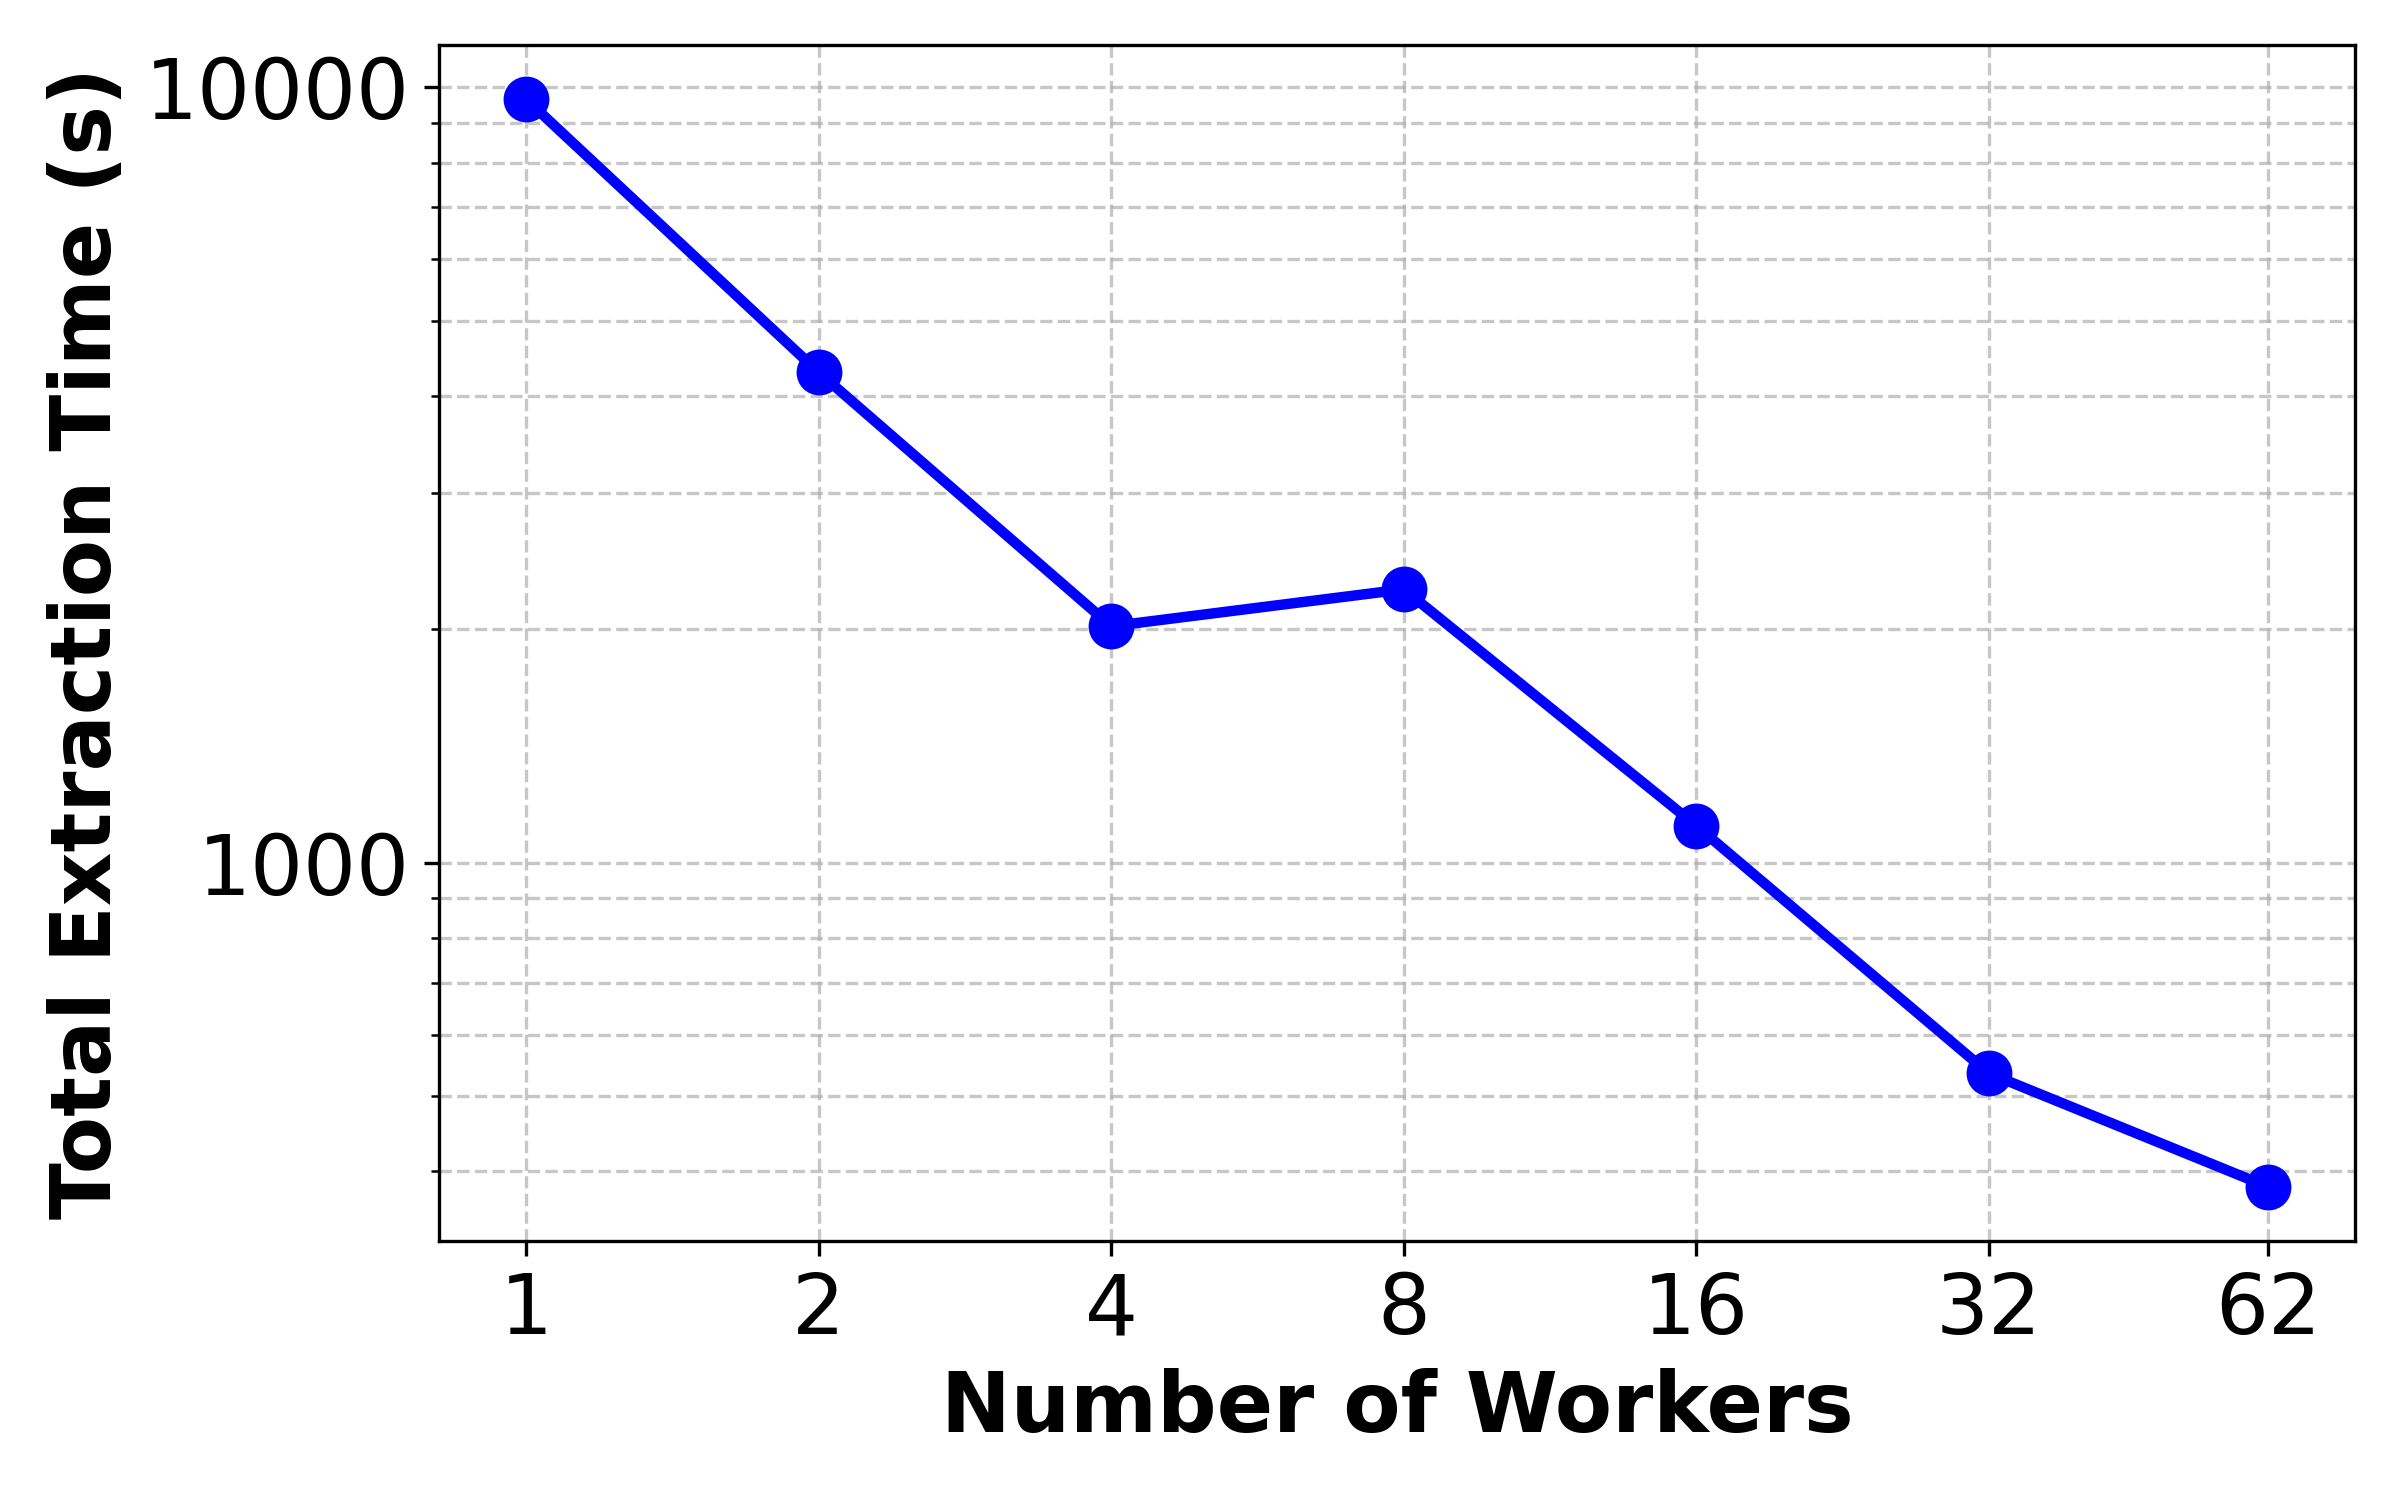
\includegraphics[width=\linewidth]{figs/extraction_scaling.png}
\caption{Total extraction wall time vs.\ worker count on the 64-core
server (log y-axis). The 8-worker point is a small regression because
the chosen chunk size oversubscribes per-core caches at that worker
count.}
\label{fig:extraction-scaling}
\end{figure}

Wall time scales roughly inversely with worker count, with one
exception at 8 workers where the chosen chunk size happens to
oversubscribe per-core caches. Going from 1 to 62 workers gives a
$25.3\times$ speedup. That speedup is real but it is not practical;
a student does not have 62 cores at home. The 4-worker configuration
is the realistic consumer setting, and it still takes 2{,}018 seconds
(close to 34 minutes) for one textbook. That is below the original
sequential baseline by almost 5$\times$, but still too long for an
interactive session. The next subsection attacks the extractor itself.

\subsection{pypdfium2 Fast Path}

Even fully parallel, \texttt{docling} is overkill for plain-text
textbooks. The Silberschatz textbook has predictable numbered section
headings and few tables; layout analysis costs minutes per pass and
gives us nothing we cannot recover with a regex.

We add a second extraction backend built on \texttt{pypdfium2}. It
reads raw text from each page range without doing layout analysis,
without writing any temporary files, and without reading the master
PDF more than once: workers seek into the master PDF directly. A
short post-processor strips lines that look like table-of-contents
entries and promotes anything that looks like a numbered section
heading (``\texttt{1.2 Database-System Applications}'') to a markdown
heading (``\texttt{\#\# 1.2 Database-System Applications}'') so the
existing markdown section splitter still works. The \texttt{docling}
backend remains available for documents that genuinely need layout
analysis.

On the RTX 6000 host (4 CPU cores), full extraction drops from
2{,}018\,s with \texttt{docling} (the 4-worker number above) to
\textbf{8.66\,s} with \texttt{pypdfium2}, a roughly $\mathbf{230\times}$
improvement on this hardware. End-to-end final score on the
regenerated index is \textbf{0.606}, slightly \emph{above} the 0.592
we get with the \texttt{docling} pipeline; the regex-based heading
promotion recovers section boundaries reliably without the
layout-analysis pass. So we cut wall time by two orders of magnitude
and answer quality goes up, not down.

Compared to the original baseline (sequential single-worker
\texttt{docling} at 9{,}650\,s), \texttt{pypdfium2} with 4 workers is
roughly $\mathbf{1{,}100\times}$ faster end to end on the same
extraction task.

%% ------------------------------------------------------------
\section{Phase 2: Hardware Router and Batch Sorting}

Two small changes in the embedder reduce ingestion wall time.

\paragraph{Length-sorted batches.}
The GGUF embedder pads each batch to the longest text in that batch
before running it through the model. Random ordering wastes compute on
short texts that share a batch with one long text. We sort inputs by
length descending before batching and permute the result back to
caller order after encoding, so the FAISS index ID order is unchanged.

\paragraph{Dynamic GPU / CPU routing.}
The indexer now checks for an NVIDIA GPU (CUDA) or Apple Silicon
(Metal) at startup. When a GPU is reachable, embedding takes a
sequential path with a batch size of 32, which keeps a single
allocator owning all the VRAM. When no GPU is reachable, embedding
falls back to a CPU process pool with workers sharing the model
weights through memory-mapped I/O. This avoids the worst case where a
CPU pool fights the GPU's allocator on a mixed host.

Phase 2 wall time depends heavily on what is already cached. By
\emph{cold} we mean the first invocation after a fresh allocation,
where the 4\,B \texttt{Qwen3-Embedding} GGUF has to be paged in from
disk and the embedding cache is empty, so every chunk goes through the
model. \emph{Warm} means a subsequent run in the same shell, where the
GGUF stays in the OS page cache and the on-disk embedding cache
already has the chunks (Step 2 then becomes mostly a cache lookup at
about 4\,ms per chunk). \emph{Super-warm} is a third run where every
cache is hot.

\begin{table}[h]
\caption{Phase 2: embedding-step wall time on 2{,}664 chunks. A100 and
V100 numbers are cold (the original V100 session and the A100 baseline
both ran on a fresh allocation). RTX 6000 numbers are warm and
super-warm; we did not capture a clean cold RTX run.}
\label{tab:phase2}
\begin{tabular}{llrr}
\toprule
GPU & run & wall (s) & peak VRAM \\
\midrule
A100 (80\,GiB)     & cold       & 305    & not recorded \\
V100 (16\,GiB)     & cold       & 426    & 4.3\,GiB \\
RTX 6000 (24\,GiB) & warm       & \textbf{33.7} & 3.4\,GiB \\
RTX 6000 (24\,GiB) & super-warm & 4.5    & 3.4\,GiB \\
\bottomrule
\end{tabular}
\end{table}

The 8\,GiB VRAM cap (set via the project's VRAM cap helper) is
non-binding because the GGUF embedder is not bound by torch's
per-process memory fraction; peak VRAM lands at 3.4\,GiB on the RTX
6000 regardless of the cap.

\shivam{Pre-Phase-2 baseline (the original embedder path with
\texttt{batch\_size=8} and no length-sorting / no GPU/CPU router) was
not captured in this round, so the table reports absolute wall times
rather than a speedup over the unoptimized path. If you re-run the
original path on the same 2{,}664-chunk corpus on RTX 6000, swap that
number in here for the speedup story; the rough expectation from the
batch-size change alone is about 4x, and the router change matters
more on mixed hosts than on this allocation.}

%% ------------------------------------------------------------
\section{Phase 3: Pluggable Embedding Backends}

\subsection{The Pluggable Backend}

A 4\,B embedder is heavy. Phase 3 makes the embedder swappable so we
can compare lighter alternatives at the same call site. The indexer
talks to a single \emph{backend} interface and the user chooses which
backend to use through one keyword argument:

\begin{itemize}
\item \textbf{llama.cpp} for any GGUF model. This is the original
  4\,B \texttt{Qwen3-Embedding} path and remains the default.
\item \textbf{GPT4All} for Nomic GGUFs. Selectable acceleration
  device: CPU, CUDA, or Vulkan (the latter avoids any NVIDIA-only
  dependency and matters on non-NVIDIA silicon).
\item \textbf{HuggingFace sentence-transformers} for arbitrary
  Hugging\-Face models, including the 137\,M Nomic-v1.5 and the
  23\,M MiniLM that we evaluate below.
\end{itemize}

The four variants we compare in this paper are \texttt{qwen4b}
(llama.cpp, 4\,B), \texttt{nomic\_st} (HF, 137\,M), \texttt{minilm}
(HF, 23\,M), and \texttt{nomic\_gpt4all} (GPT4All, 137\,M).

% \subsection{Two Adjacent Fixes}

% \paragraph{BLEU.}
% The original metric suite had semantic and keyword similarity but no
% n-gram surface-overlap signal, so two answers that mean the same
% thing at different paraphrase strengths could not be distinguished. We
% add a sentence-level BLEU-4 metric (NIST method-1 smoothing) so the
% final-score weighting in Section~\ref{sec:metrics} can include surface
% overlap.

% \paragraph{The pollution bug.}
% The semantic-similarity scorer (an MPNet model used to compare each
% generated answer to the reference) was forcing CPU mode for itself by
% clearing the CUDA-visibility environment variable at import time. That
% clearing was process-wide, so it also disabled the GPU for everything
% else started later in the same Python process, including the answer
% generator. End-to-end test wall on a V100 dropped from about 700\,s to
% about 45\,s once we left CUDA visible to the rest of the suite and
% pinned only the scoring model to CPU. The bug was easy to miss because
% the suite kept passing on quality; it just ran 15$\times$ slower than
% it should have.

\subsection{Quality Comparison on V100}

Table~\ref{tab:phase3-v100} reports all four metrics from
Section~\ref{sec:metrics} on the four variants, on a V100 with a fresh
allocation.

\begin{table}[h]
\caption{Phase 3, V100, 11-question benchmark suite. All numbers
are means over the 11 benchmarks. Higher is better.}
\label{tab:phase3-v100}
\begin{tabular}{lrrrrr}
\toprule
variant & params & sem & kw & BLEU & final \\
\midrule
qwen4b              & 4\,B   & 0.761 & 0.310 & 0.026 & 0.592 \\
nomic\_st           & 137\,M & 0.735 & \textbf{0.346} & \textbf{0.032} & 0.589 \\
\textbf{minilm}     & 23\,M  & \textbf{0.778} & 0.310 & 0.026 & \textbf{0.603} \\
nomic\_gpt4all      & 137\,M & 0.716 & 0.295 & 0.026 & 0.558 \\
\bottomrule
\end{tabular}
\end{table}

The 23\,M MiniLM variant takes the top final score (0.603), with the
4\,B Qwen baseline second (0.592) and the 137\,M sentence-transformers
Nomic third (0.589). MiniLM also wins on semantic similarity (0.778)
because its short sentence embeddings happen to align well with the
MPNet scorer's notion of similarity. Sentence-transformers Nomic wins
on keyword similarity (0.346) and BLEU (0.032), which means it pulls
in answer text that copies more of the reference's vocabulary
verbatim. The GPT4All variant is the weakest of the four on every
metric (final 0.558), almost entirely because of one benchmark
(\texttt{book\_authors}) where its retrieval pulls a near-empty chunk
and the generator returns a malformed answer that scores 0.07 on
final.

A 23\,M model beating a 4\,B model on a final-score weighted toward
semantic similarity looks surprising. The reason is the cross-encoder
reranker downstream. The reranker re-scores the FAISS top-50
candidates against the actual question text and picks the top 5 to
prompt the generator. As long as the right chunk is somewhere in the
top 50, the reranker can find it; the embedder just has to be good
enough to keep the right chunk in candidate range. On a small corpus
like this textbook, even a 23\,M embedder clears that bar for most
questions.

%% ------------------------------------------------------------
\section{Consumer-GPU Evaluation}

The headline question is whether the system runs end to end on a
consumer GPU at the 8\,GiB cap. We answer it on the RTX 6000 with the
VRAM cap helper enabling
\texttt{torch.cuda.set\_per\_process\_memory\_fraction(8/24)} for any
torch process in the run. The GGUF embedder is not bound by torch's
allocator, so for that variant we report natural peak VRAM and confirm
it stays under 8\,GiB on its own.

\subsection{What the Wall Time Includes}

The wall column in Table~\ref{tab:rtx-capped} is end-to-end pytest
time for the 11-question benchmark suite on a single variant: per-query
embedding, FAISS+BM25 retrieval, cross-encoder rerank, Qwen2.5-1.5B
answer generation, and metric scoring. It \emph{does not} include the
one-time index build (Phase 2 above), since the index is built once
per corpus and reused across queries. All runs are warm, the second
invocation after the index already exists.

\subsection{Results}

\begin{table}[h]
\caption{Phase 3, RTX 6000, \texttt{VRAM\_CAP\_GIB=8}. Wall time is
the full 11-question pytest loop per variant. Final score uses the
metrics defined in Section~\ref{sec:metrics}.}
\label{tab:rtx-capped}
\begin{tabular}{lrrr}
\toprule
variant & wall (s) & peak VRAM (MiB) & final \\
\midrule
minilm                       & \textbf{40.3} & 2{,}214 & 0.578 \\
nomic\_st                    & 36.2 & 2{,}706 & 0.563 \\
qwen4b                       & 37.1 & 5{,}392 & 0.592 \\
nomic\_gpt4all\_gpu & 36.2 & \textbf{2{,}124} & 0.558 \\
\bottomrule
\end{tabular}
\end{table}

The largest peak is 5.4\,GiB (the 4\,B baseline). Every other variant
uses less than 3\,GiB. Final scores match the uncapped run because the
cap only reserves VRAM and does not change numerics. The Vulkan
(kompute) path used by the GPT4All backend has the smallest VRAM
footprint of the four (2.1\,GiB) and provides a CUDA-free option for
non-NVIDIA silicon.

%% ------------------------------------------------------------
\section{Code and Artifacts}

The full code is available at
\url{https://github.com/singhals163/TokenSmith}. Each optimization
lives on its own branch so the diff against \texttt{main} is small
enough to read independently. The branches relevant to this
submission are:

\begin{description}
\item[\texttt{feat/parallel-extraction}] Phase 1, the docling
  map-reduce extractor.
\item[\texttt{feat/pypdfium-extractor}] Phase 1.5, the
  \texttt{pypdfium2} fast extraction path.
\item[\texttt{feat/embedder-router}] Phase 2, the GPU/CPU routing and
  length-sorted batches.
\item[\texttt{feat/pluggable-embedders}] Phase 3, the pluggable
  embedder backend (\texttt{llama.cpp} / GPT4All /
  \texttt{sentence-transformers}) plus the BLEU metric and the
  GPU-pollution fix.
\item[\texttt{tools}] Helper code used to gather the numbers in this
  paper (profiler, VRAM cap helper, per-variant index and pytest
  drivers).
\item[\texttt{experiments}] All four feature branches integrated, the
  per-experiment result artifacts under \texttt{experiments/}, and a
  markdown version of this writeup (\texttt{REPORT.md}).
\end{description}

%% ------------------------------------------------------------
\section{Conclusion}

Four targeted changes bring TokenSmith from a server-class system to
one that runs in 40 seconds on a 4-core / 8-GiB profile without losing
answer quality. The 23\,M MiniLM variant matches the 4\,B baseline
within 1.4 points on final score; the 4\,B baseline still runs and
remains the highest-quality option for users who can spare the time.
The system is no longer bottlenecked on GPU memory at this profile;
the remaining latency floor is cold extraction, which the
\texttt{pypdfium2} fast path addresses. The full code is organized
as one branch per feature on the project's git remote, with a separate
branch for the helper scripts and another holding the per-experiment
artifacts.

\end{document}
